\documentclass{standalone}
\usepackage{tikz}
\usepackage{ctex,siunitx}
\setCJKmainfont{Noto Serif CJK SC}
\usepackage{tkz-euclide}
\usepackage{amsmath}
\usetikzlibrary{patterns, calc}
\usetikzlibrary {decorations.pathmorphing, decorations.pathreplacing, decorations.shapes,}

\begin{document}
\small
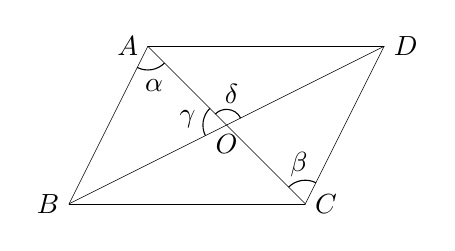
\begin{tikzpicture}[>=stealth,scale=1.0]
  \tkzSetUpPoint[fill=black]
  % \useasboundingbox(-1,-0.75)rectangle(3.7,1.4);
  \tkzDefPoints{0/0/B, 3/0/C, 1/2/A, 4/2/D,2/1/O}
  \tkzDrawSegments(B,C A,B A,C C,D A,D B,D)
  \tkzLabelPoints[below](O)	  
  \tkzLabelPoints[left](A,B)	
  \tkzLabelPoints[right](C,D)	
  \tkzMarkAngles[mark=none, size=.3](B,A,C A,O,B D,C,A)
  \tkzMarkAngles[mark=none, size=.2](D,O,A)
  \tkzLabelAngle[pos=.5](B,A,C){$\alpha$}
  \tkzLabelAngle[pos=.5](A,O,B){$\gamma$}
  \tkzLabelAngle[pos=.5](D,C,A){$\beta$}
  \tkzLabelAngle[pos=.4](D,O,A){$\delta$}
\end{tikzpicture}
\end{document}